\documentclass{csse4400}

% \teachermodetrue

\usepackage{float}

\usepackage{languages}

\title{Application Programming Interfaces (APIs)}
\author{Brae Webb}

\date{\week{5}}
\begin{document}

\maketitle

\begin{figure}[h]
  \href{https://www.oreilly.com/library/view/designing-data-intensive-applications/9781491903063/ch04.html}{
    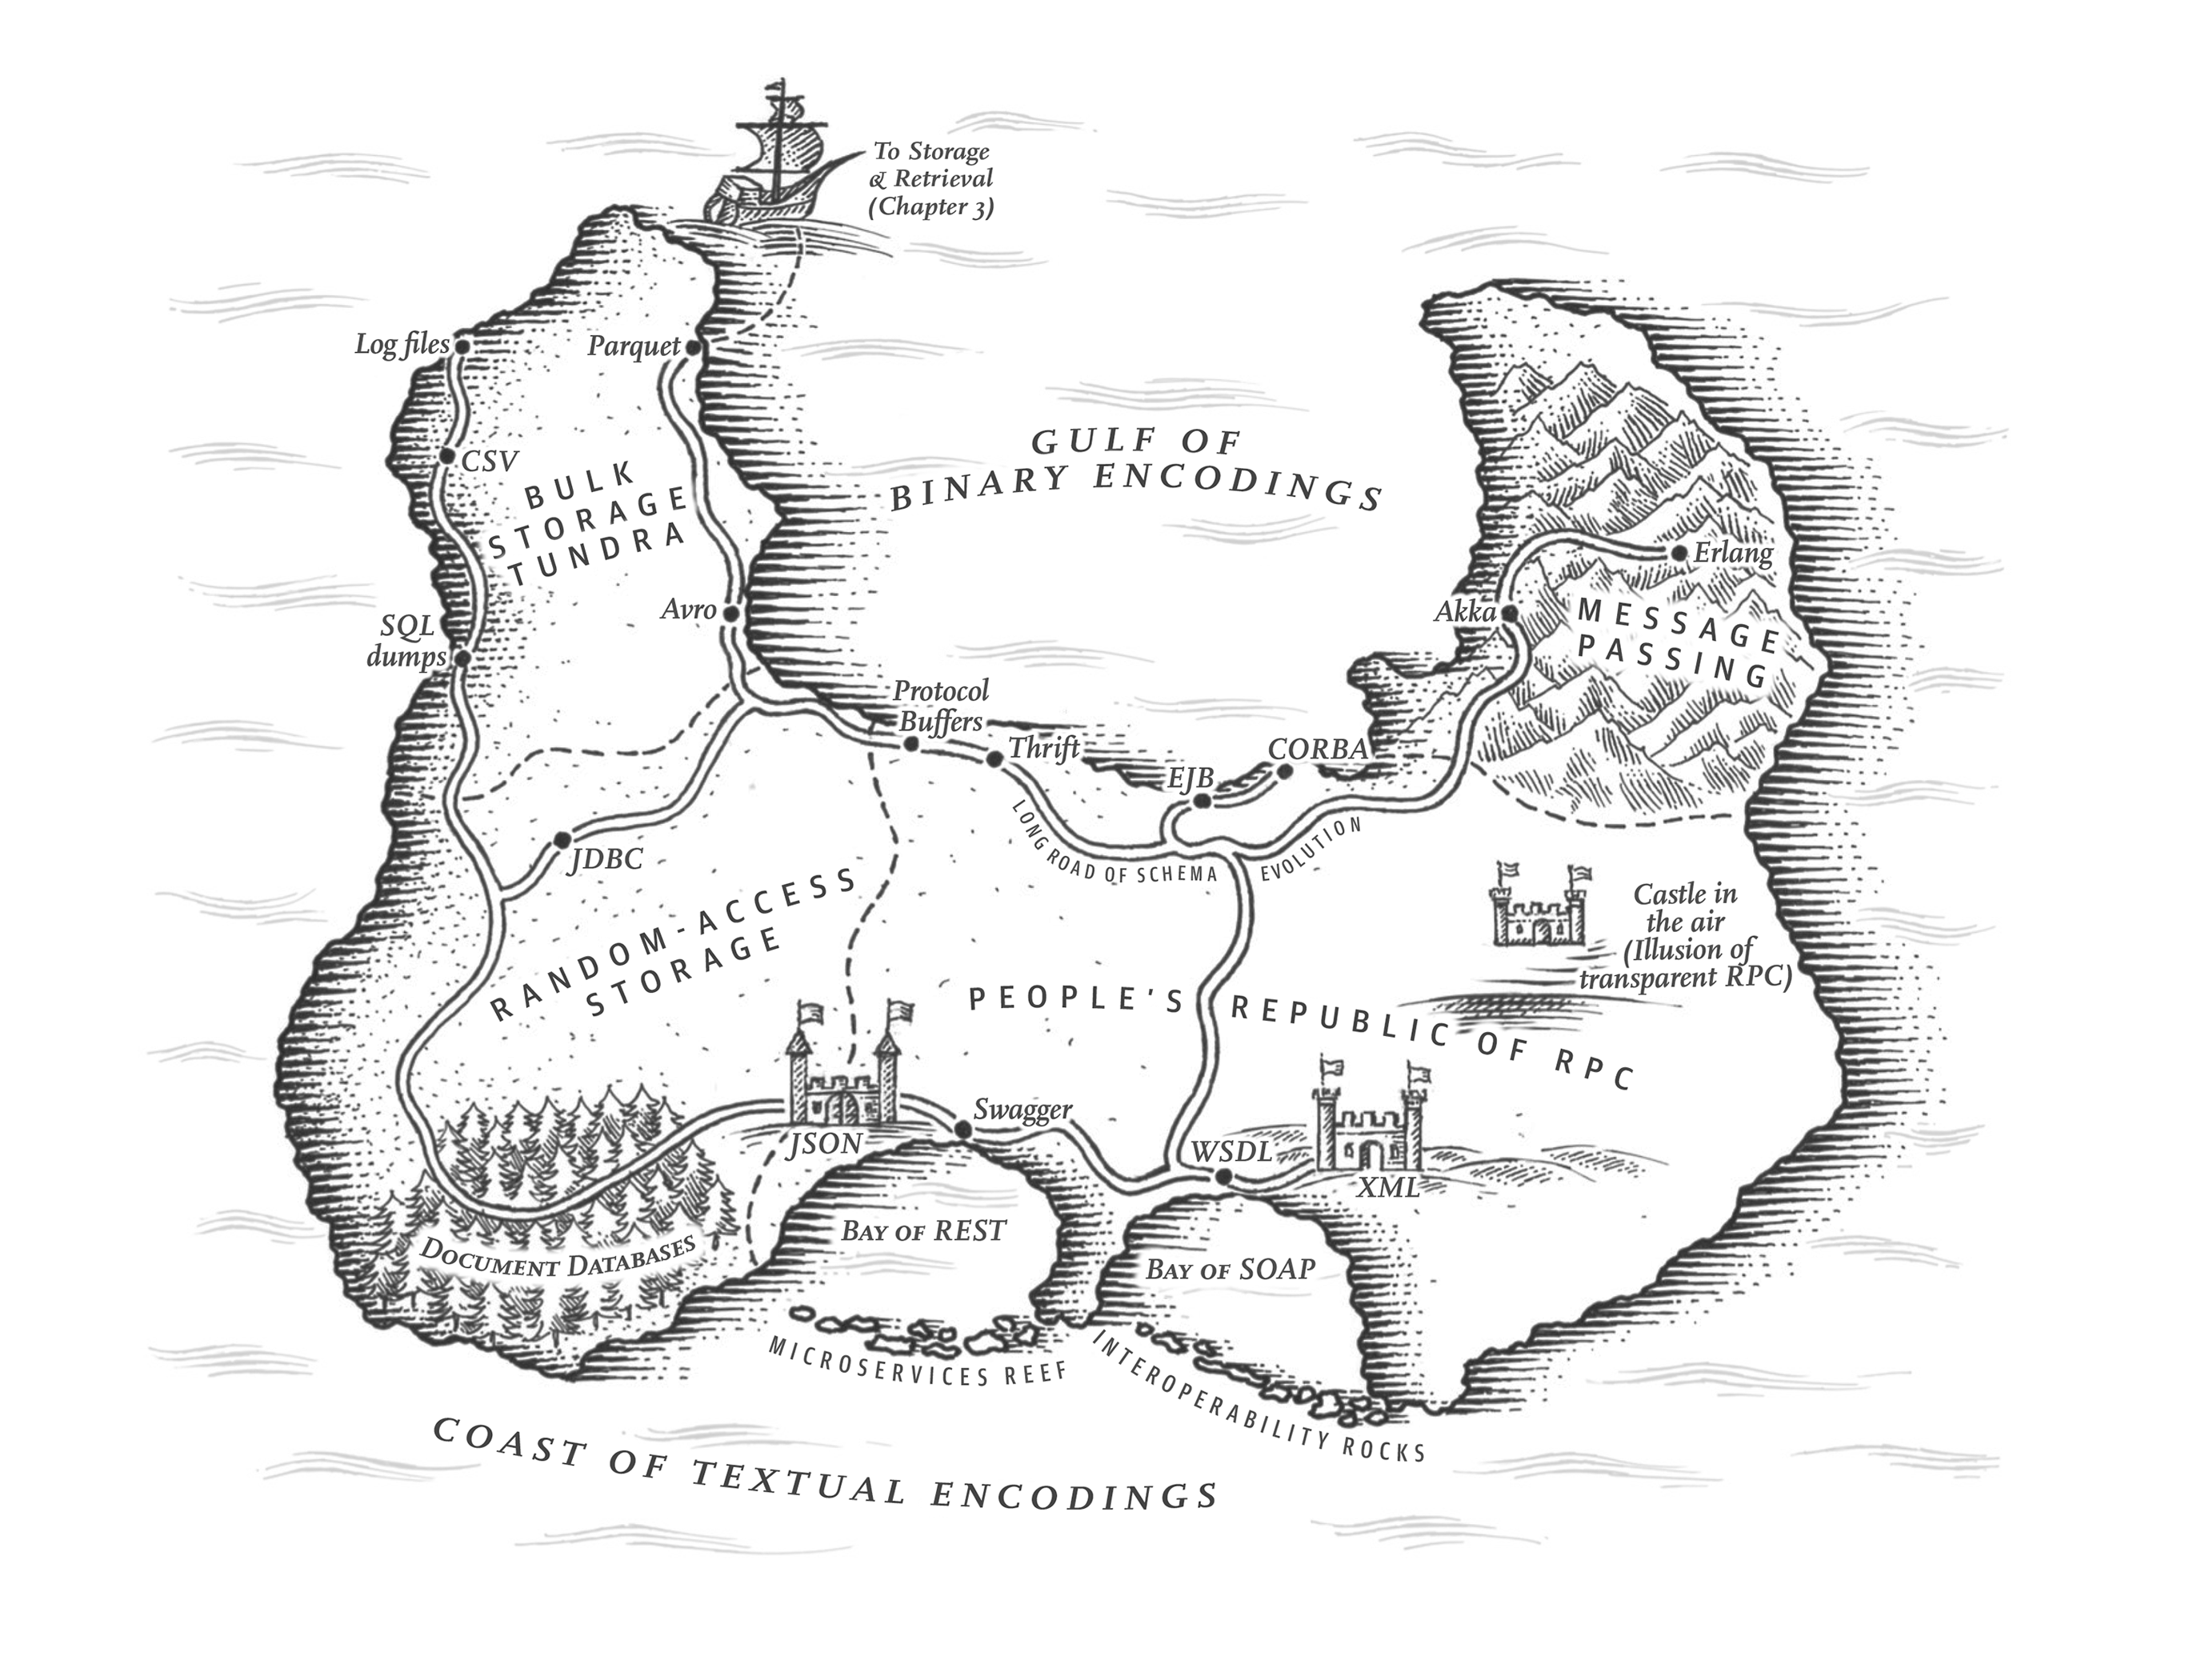
\includegraphics[width=\textwidth]{images/communication}
  }
\caption{A map of communication techniques from Designing Data-Intensive Applications \cite{data-intensive}.}
\end{figure}

\section{This Week}
This week our goal is to:
\begin{itemize}
  \item explore the various techniques developers use to communicate between distributed systems;
  \item deploy a static website on an S3 bucket; and
  \item configure the static website to communicate with the EC2 backend.
\end{itemize}

\teacher{
    As with last week, spend approximately the first 30 minutes exploring concepts.
}

\section{Communication}
This week we have started to explore the world of distributed systems.
The world relies (heavily) on distributed systems,
there is no machine in the world powerful enough to process the requests Google receives every second.
We need to have many hundreds of machines working seamlessly together.
This inter-machine teamwork requires machines to know how to talk to each other.
For the practical this week we will look at APIs as a mechanism for communication.

\section{Data Formats}
When engaging in communication we wish to exchange information.
On computer systems information is stored at runtime in memory as primitive data which your programming language can interpret;
bytes, integers, strings, etc.
In object-oriented languages,
primitive data is wrapped up into useful packages: objects.
If we want this information to escape the confines of our programming language runtime,
we need to package it up in a language-independent format.
For a format to be language-independent we just need many languages to implement an encoding and decoding mechanism for the format.
We have a number of language-independent formats available but a few defacto standards.

\subsection{XML}
Extensible Markup Language (XML) is one of the most widely used language-independent formats.
The use cases of XML are extensive,
it's the \link{foundation for many popular utilities}{https://en.wikipedia.org/wiki/List_of_XML_markup_languages},
such as SVG file formats, SAML authentication, RSS feeds, and ePub books.

\begin{code}[language=xml]{csse6400.xml}
<root>
  <item>
    <key>Course Code</key>
    <value>CSSE6400</value>
  </item>
  <item>
    <key>Course Title</key>
    <value>Software Architecture</value>
  </item>
</root>
\end{code}

XML is designed as a markup language, similar to HTML,
it is not designed as a data exchange format.
Developers have come to point out that the verbosity and complexity of XML,
compared to alternatives such as JSON, are deal breakers.
While XML can be used as a data exchange format it is not designed for it,
and as a result APIs built around XML as a data format are becoming less common.

\subsection{JSON}
JavaScript Object Notation (JSON) is quickly replacing XML as the data format used in APIs.
As you will note, it is more succinct and communicates the important points to a human reader better.
Although the popularity of JSON is largely due to the compatibility with JavaScript which has taken over web development.
JSON is the map-esque data type in JavaScript.
Detractors of JSON claim that it's main disadvantage over XML is that it lacks a schema.
However, \link{schemas are possible in JSON}{https://json-schema.org/},
they are optional,
just as in XML but much less used than XML.

\begin{code}[language=json]{csse6400.json}
{
    "Course Code": "CSSE6400",
    "Course Title": "Software Architecture"
}
\end{code}

\subsection{MessagePack}
It should not be a surprise that the JSON and XML formats are not resource efficient.
Nowadays, we are less concerned with squeezing data into a tiny amount of data on the hard drive as our hard drives are massive.
However, we are often concerned with how much data is being transmitted via network communication.

In the example JSON snippet above, we use 78 bytes to encode the message.
\link{MessagePack}{https://msgpack.org/} is a standard for encoding and decoding JSON.
When encoding our original JSON snippet with MessagePack we shrink to just 57 bytes.
At our scale, a negligible difference,
but at the scale of terrabytes or petabytes,
a significant consideration.

\begin{code}[]{csse6400.msgpack}
82 ab 43 6f 75 72 73 65 20 43 6f 64 65 a8 43 53 53 45 36 34 30 30 ac 43 6f 75 72 73 65 20 54 69 74 6c 65 b5 53 6f 66 74 77 61 72 65 20 41 72 63 68 69 74 65 63 74 75 72 65
\end{code}

\info{
    For those interested,
    0x82 specifies a map type (0x80) with two fields (0x02).
    Followed by a string type (0xa0) of size eleven (0x0b).
    The rest is left as an exercise: \url{https://github.com/msgpack/msgpack/blob/master/spec.md}.
}

\subsection{Protobuf}
Protocol Buffers (protobuf) is another type of binary encoding.
However, unlike MessagePack, the format was designed from scratch,
allowing a more compact and better designed format.
Protobufs require all data to be defined by a schema.
For example:

\begin{code}[language=protobuf]{csse6400.proto}
message Course {
    required string code = 1;
    required string name = 2;
}
\end{code}

Protobufs differ from XML, JSON, and MessagePack via their method of integration.
In all other examples,
your language would have a library to encode and decode the data format into and out of your languages type system.
With protobuf, an external tool, \textsl{protoc},
takes the schema and generates a model of the schema in your target language.
This gives every language a native method to interact with the data format,
it often means that developers don't need to be aware of the underlying encoding.

\begin{code}[language=java]{csse6400.java}
Course softarch = Course.newBuilder()
    .setCode("CSSE6400")
    .setName("Software Architecture")
    .build();
output = new FileOutputStream(args[0]);
softarch.writeTo(output);
\end{code}

\section{Application Programming Interfaces}
\subsection{XML-RPC}
\subsection{SOAP}
\subsection{REST}
\subsection{JSON-RPC}
\subsection{GraphQL}
\subsection{gRPC}

\section{Deploying a Todo Part Two}

In the practical last week we deployed a very simple todo application.
Recall that we deployed a database and an EC2 instance which acted as a docker container.
The EC2 instance was responsible for:
\begin{enumerate}
  \item allowing users to download the client-side HTML and Javascript frontend; and
  \item providing a REST API the client talked to in order to access persistent data.
\end{enumerate}
This means that each time the client opens the website they will need to download the frontend and make all subsequent requests to the same instance.
This doesn't scale well.
In this practical, we will make one simple change that helps increase our capacity.

The todo application was built using a simple layered architecture.
\begin{enumerate}
  \item The client-side (or presentation layer) is developed in \link{Elm}{https://elm-lang.org/} which compiles into static HTML and JavaScript.
  \item The presentation layer communicates with a \link{Laravel}{https://laravel.com/} persistence layer via a REST API.
  \item The persistence layer in turn communicates with a \link{MySQL}{https://www.mysql.com/} database layer.
\end{enumerate}

We have already deployed the database layer separately from the presentation and persistence layer.
Now, we want to deploy the service which serves the presentation layer separately from the persistence layer.
Since our presentation layer is static,
we can take advantage of the AWS S3 service.
AWS S3 is scalable, which means that we don't have to worry about manually scaling our frontend serving (and can focus on the challenging of backend scaling).

\begin{figure}[ht]
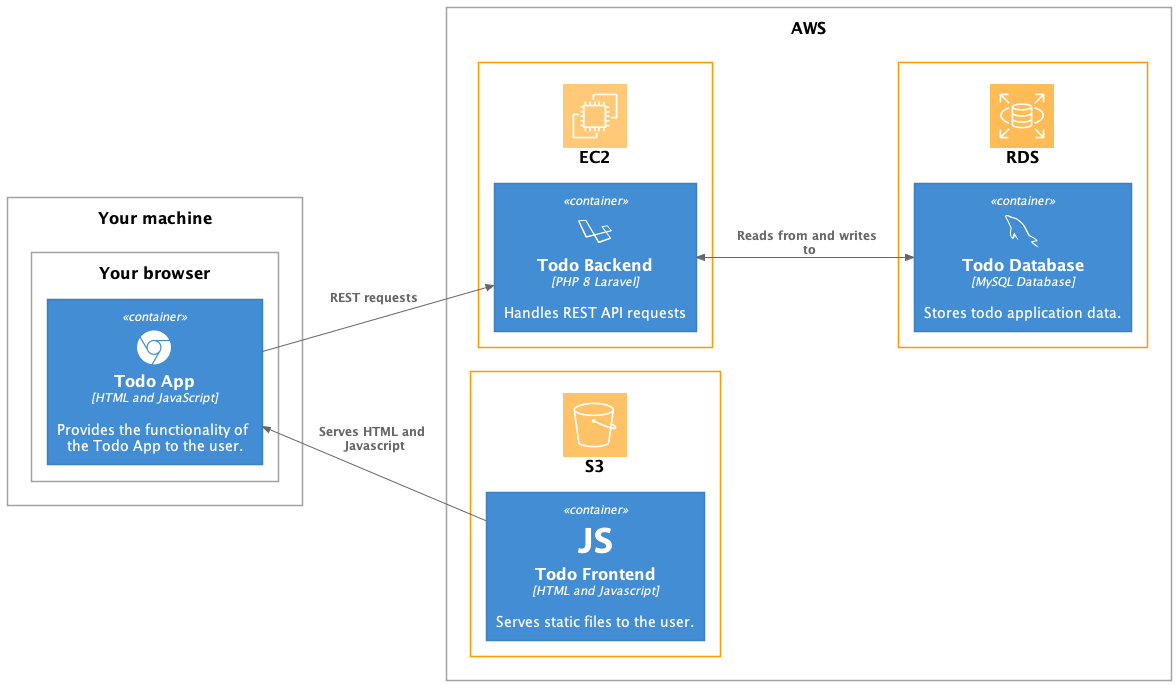
\includegraphics[width=\textwidth]{diagrams/deployment}
\caption{Desired deployment diagram of the todo application.}
\end{figure}

\bibliographystyle{ieeetr}
\bibliography{books,ours}

\end{document}